\chapter{Application}\label{chpt:application}
\glsresetall

This chapter is about the application that was motivated in section~\ref{sec:intro:problem}. First of 
all the concept is specified. After that the acquisition of data as well as the implementation of the 
different components is described.

\section{Concept}\label{sec:app:concept}

The following concept is divided into two parts. The first part describes the productive application 
that transforms a Valorant video into another data representation using a pattern recognition 
algorithm. The second part covers all workflows to train a machine learning model that is used in the 
first part.

\subsection{Inference Application}\label{subsec:app:inference}

The productive application consists of five elements:

\begin{itemize}
	\item[\textbf{I1:}] Raw data
	\item[\textbf{I2:}] Data pre-processing
	\item[\textbf{I3:}] Neural network model
	\item[\textbf{I4:}] Post-processing algorithm
	\item[\textbf{I5:}] Transformed data representation
\end{itemize}

As raw data (I1) videos with Valorant gameplay are used. Those videos show a screen as depicted in 
figure~\ref{fig:intro:ingame}. Within this project the goal is to derive an alternative data 
representation (I5) that helps players and trainers getting a better overview of single rounds. 
Therefore it is important that the videos just show individual rounds and not a whole match. This is 
secured in the data pre-processing step (I2). In order to generate a new representation that gives an 
overview, the data over time is summarized and presented as a single image, like that in 
figure~\ref{fig:app:output}. However, only the information from the minimap in the upper left corner 
of the video is sufficient and due to training reasons, which are discussed in 
section~\ref{subsec:app:training}, this part of the map is also extracted during pre-processing (I2). 
The further steps are only performed on the cropped part of the video.

\begin{figure}
	\centering
	\includegraphics[width=0.8\linewidth]{images/05-output}
	\caption[Output representation as map.]{Output representation as map, summarizing all positions 
	of defender agents in one round on the map "Haven".}
	\label{fig:app:output}
\end{figure}

Image~\ref{fig:intro:minimap} shows different entities that could be target of the detection 
algorithm~(I3). One possibility is just to find all defender agents without distinguishing the specific 
agent. The result of such an analysis is shown in figure~\ref{fig:app:output}. This is a graph that 
summarizes all positions of the defending team on the already mentioned map "Haven". In a more 
advanced approach it is possible to detect the specific agents and create motion profiles for 
each of them. In addition, team or opponent abilities could also be recognized. It would be possible 
as well to combine those detection tasks and then create various views to present the gathered 
data. In order to generate evaluation data a model of a neural network (I3) is needed. This is trained 
by the application described in section~\ref{subsec:app:training}. Finally a post-processing 
algorithm (I4) transforms the output data from the neural network into a better recognizable form of 
presentation (I5).

\subsection{Training Application}\label{subsec:app:training}



\begin{figure}
	\centering
	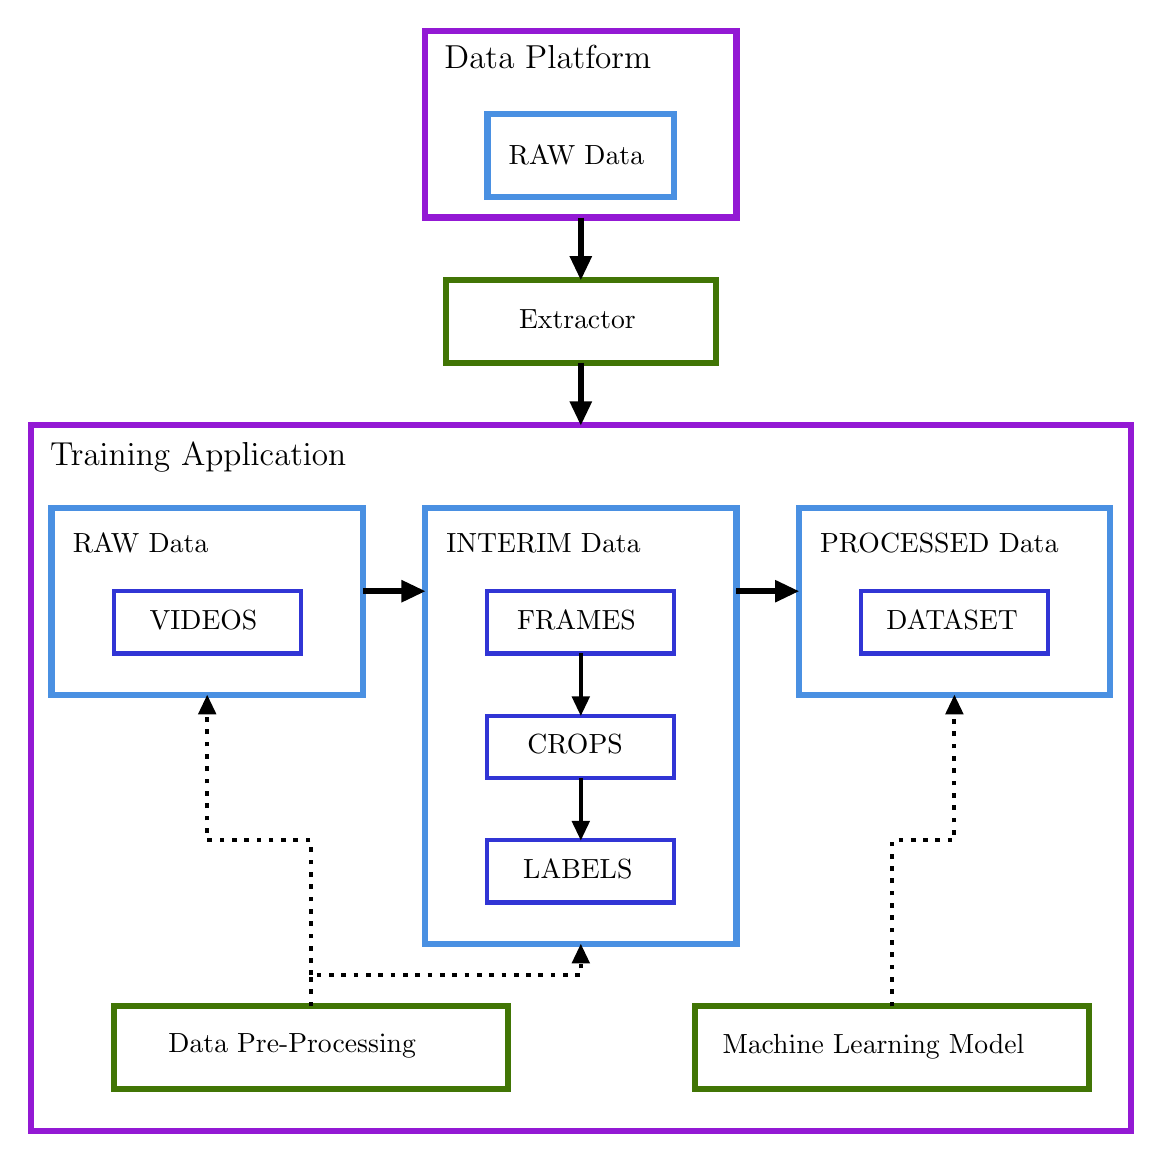
\begin{tikzpicture}[x=0.75pt,y=0.75pt,yscale=-1,xscale=1]
		\draw  [color={rgb, 255:red, 147; green, 25; blue, 212 }  ,draw opacity=1 ][line width=2.25]  
		(250,10) -- (400,10) -- (400,100) -- (250,100) -- cycle ;
		\draw  [color={rgb, 255:red, 147; green, 25; blue, 212 }  ,draw opacity=1 ][line width=2.25]  
		(60,200) -- (590,200) -- (590,540) -- (60,540) -- cycle ;
		\draw  [color={rgb, 255:red, 65; green, 117; blue, 5 }  ,draw opacity=1 ][line width=2.25]  
		(260,130) -- (390,130) -- (390,170) -- (260,170) -- cycle ;
		
		\draw [line width=2.25]    (325,100) -- (325,125) ;
		\draw [shift={(325,130)}, rotate = 270] [fill={rgb, 255:red, 0; green, 0; blue, 0 }  ][line 
		width=0.08]  [draw opacity=0] (11.43,-5.49) -- (0,0) -- (11.43,5.49) -- cycle    ;
		\draw [line width=2.25]    (325,170) -- (325,195) ;
		\draw [shift={(325,200)}, rotate = 270] [fill={rgb, 255:red, 0; green, 0; blue, 0 }  ][line 
		width=0.08]  [draw opacity=0] (11.43,-5.49) -- (0,0) -- (11.43,5.49) -- cycle    ;
		\draw  [color={rgb, 255:red, 74; green, 144; blue, 226 }  ,draw opacity=1 ][line width=2.25]  
		(70,240) -- (220,240) -- (220,330) -- (70,330) -- cycle ;
		\draw  [color={rgb, 255:red, 74; green, 144; blue, 226 }  ,draw opacity=1 ][line width=2.25]  
		(280,50) -- (370,50) -- (370,90) -- (280,90) -- cycle ;
		
		\draw  [color={rgb, 255:red, 65; green, 117; blue, 5 }  ,draw opacity=1 ][line width=2.25]  
		(100,480) -- (290,480) -- (290,520) -- (100,520) -- cycle ;
		
		\draw  [color={rgb, 255:red, 74; green, 144; blue, 226 }  ,draw opacity=1 ][line width=2.25]  
		(250,240) -- (400,240) -- (400,450) -- (250,450) -- cycle ;
		\draw  [color={rgb, 255:red, 49; green, 53; blue, 213 }  ,draw opacity=1 ][line width=1.5]  
		(100,280) -- (190,280) -- (190,310) -- (100,310) -- cycle ;
		\draw  [color={rgb, 255:red, 49; green, 53; blue, 213 }  ,draw opacity=1 ][line width=1.5]  
		(280,280) -- (370,280) -- (370,310) -- (280,310) -- cycle ;
		
		\draw  [color={rgb, 255:red, 49; green, 53; blue, 213 }  ,draw opacity=1 ][line width=1.5]  
		(280,340) -- (370,340) -- (370,370) -- (280,370) -- cycle ;
		
		\draw  [color={rgb, 255:red, 49; green, 53; blue, 213 }  ,draw opacity=1 ][line width=1.5]  
		(280,400) -- (370,400) -- (370,430) -- (280,430) -- cycle ;
		
		\draw [line width=1.5]    (325,310) -- (325,336) ;
		\draw [shift={(325,340)}, rotate = 270] [fill={rgb, 255:red, 0; green, 0; blue, 0 }  ][line 
		width=0.08]  [draw opacity=0] (9.29,-4.46) -- (0,0) -- (9.29,4.46) -- cycle    ;
		\draw [line width=1.5]    (325,370) -- (325,396) ;
		\draw [shift={(325,400)}, rotate = 270] [fill={rgb, 255:red, 0; green, 0; blue, 0 }  ][line 
		width=0.08]  [draw opacity=0] (9.29,-4.46) -- (0,0) -- (9.29,4.46) -- cycle    ;
		\draw [line width=2.25]    (220,280) -- (245,280) ;
		\draw [shift={(250,280)}, rotate = 180] [fill={rgb, 255:red, 0; green, 0; blue, 0 }  ][line 
		width=0.08]  [draw opacity=0] (11.43,-5.49) -- (0,0) -- (11.43,5.49) -- cycle    ;
		\draw  [color={rgb, 255:red, 74; green, 144; blue, 226 }  ,draw opacity=1 ][line width=2.25]  
		(430,240) -- (580,240) -- (580,330) -- (430,330) -- cycle ;
		\draw  [color={rgb, 255:red, 49; green, 53; blue, 213 }  ,draw opacity=1 ][line width=1.5]  
		(460,280) -- (550,280) -- (550,310) -- (460,310) -- cycle ;
		
		\draw [line width=2.25]    (400,280) -- (425,280) ;
		\draw [shift={(430,280)}, rotate = 180] [fill={rgb, 255:red, 0; green, 0; blue, 0 }  ][line 
		width=0.08]  [draw opacity=0] (11.43,-5.49) -- (0,0) -- (11.43,5.49) -- cycle    ;
		\draw  [color={rgb, 255:red, 65; green, 117; blue, 5 }  ,draw opacity=1 ][line width=2.25]  
		(380,480) -- (570,480) -- (570,520) -- (380,520) -- cycle ;
		
		\draw [line width=1.5]  [dash pattern={on 1.69pt off 2.76pt}]  (195,480) -- (195,465) -- 
		(325,465) -- (325,454) ;
		\draw [shift={(325,450)}, rotate = 90] [fill={rgb, 255:red, 0; green, 0; blue, 0 }  ][line 
		width=0.08]  [draw opacity=0] (9.29,-4.46) -- (0,0) -- (9.29,4.46) -- cycle    ;
		\draw [line width=1.5]  [dash pattern={on 1.69pt off 2.76pt}]  (195,465) -- (195,400) -- 
		(145,400) -- (145,334) ;
		\draw [shift={(145,330)}, rotate = 90] [fill={rgb, 255:red, 0; green, 0; blue, 0 }  ][line 
		width=0.08]  [draw opacity=0] (9.29,-4.46) -- (0,0) -- (9.29,4.46) -- cycle    ;
		\draw [line width=1.5]  [dash pattern={on 1.69pt off 2.76pt}]  (475,480) -- (475,400) -- 
		(505,400) -- (505,334) ;
		\draw [shift={(505,330)}, rotate = 90] [fill={rgb, 255:red, 0; green, 0; blue, 0 }  ][line 
		width=0.08]  [draw opacity=0] (9.29,-4.46) -- (0,0) -- (9.29,4.46) -- cycle    ;
		
		\draw (258,16) node [anchor=north west][inner sep=0.75pt]   [align=left] {{\large Data 
		Platform}};
		\draw (68,207) node [anchor=north west][inner sep=0.75pt]   [align=left] {{\large Training 
		Application}};
		\draw (289,64) node [anchor=north west][inner sep=0.75pt]   [align=left] {RAW Data};
		\draw (294,143) node [anchor=north west][inner sep=0.75pt]   [align=left] {Extractor};
		\draw (79,251) node [anchor=north west][inner sep=0.75pt]   [align=left] {RAW Data};
		\draw (259,251) node [anchor=north west][inner sep=0.75pt]   [align=left] {INTERIM Data};
		\draw (439,251) node [anchor=north west][inner sep=0.75pt]   [align=left] {PROCESSED Data};
		\draw (392,492) node [anchor=north west][inner sep=0.75pt]   [align=left] {Machine Learning 
		Model};
		\draw (116,288) node [anchor=north west][inner sep=0.75pt]   [align=left] {VIDEOS};
		\draw (471,288) node [anchor=north west][inner sep=0.75pt]   [align=left] {DATASET};
		\draw (293,288) node [anchor=north west][inner sep=0.75pt]   [align=left] {FRAMES};
		\draw (298,348) node [anchor=north west][inner sep=0.75pt]   [align=left] {CROPS};
		\draw (296,408) node [anchor=north west][inner sep=0.75pt]   [align=left] {LABELS};
		\draw (125,492) node [anchor=north west][inner sep=0.75pt]   [align=left] {Data 
		Pre-Processing};
	\end{tikzpicture}
	\caption{Concept for the training application.}
	\label{fig:app:conceptTrain}
\end{figure}

\section{Data}\label{sec:app:data}

\section{YOLOv5}\label{sec:app:yolov5}

\section{Implementation}\label{sec:app:impl}

\section{Dataset}\label{sec:app:dataset}

\section{Summary}\label{sec:app:summary}
